\chapter{Scalability techniques}
\label{ch:Scalability Techniques}

This chapter discusses three types of scalability techniques that could be adopted in any of the scalability approaches which are discussed in the chapter \ref{ch:Scalability Approaches}.

\section{Service replication}

A technique to clone services running on other nodes to stabilize the service load among different nodes without causing any damage to the ongoing operations. Services that are replicated secure additional resources provided by the new nodes for handling larger service load. In other words, service replication enhances service scalability and reduces the risk of QoS degradation by handling larger service loads. In a case study, Falatah and Omar \cite{falatah_cloud_2014}, performed an analysis by varying the system load. Firstly, a variable for service load is set. The service load is a number of service invocations within a unit time. For the case study, the unit time was set to be 500ms. That is, if ten invocations occur within 500ms, then the service load is 10. To show an effectiveness of service replication, they simulate the service replication scheme for seventeen different volumes of service load. On each service load, conventional service system is compared with service replication strategy in terms of average response time.

Service replication is easier when the server is stateless, but the MANO will have a database, user session and various managed services. Simply replicating servers cannot be the solution as multiple MANOs using a single database will lead to a bottleneck. Hence, database clustering or database replication is also needed to maintain uniformity across the databases.  
Service replication increases availability and parallelism.


\section{Service migration}

Service migration is a strategy of placing a service on a different node when a particular node cannot provide high QoS due to a hardware/software problem or due to the physical distance between consumers and providers. After service migration, the migrated service performs the same role that it was supposed to performed on the unstable node and the unstable node is removed from the list of service nodes.
The removal of this unstable node reduces overall QoS degradation.
Lee and Kim \cite{lee_software_2010} conducted a simulation where the service was migrated to a node that is located closer to consumer. There is also an assumption made that the response time is directly proportional to the distance. Hence, a service is migrated to the fastest node in terms of response time.

In terms of MANO, it manages VIMs in different locations. There is a close association between MANOs and VIMs to handle the lifecycle management of an NS.
Mere migration of a MANO server closer to the operator will not make the communication time between MANO and VIM faster. Instead, migrating the instance of MANO closer to the VIMs will improve the overall NS lifecycle management time.

\section{Service system scaling - dynamic node scaling}

To scale a distributed system with nodes spread over different locations, management components which help in monitoring the status of all these nodes are needed. Lee and Kim \cite{lee_software_2010} propose two key components to manage service scalability, Global Scalability Manager (GSM) and Regional Scalability Manager (RSM).

The key role of GSM is to manage service scalability. It balances service load in the system by obtaining the current status of nodes that are listed in the service system and designs a scalability strategy.

RSM component is installed on all the service nodes. It observes the status of its node and communicates it to the GSM. RSM also executes the scalability strategy based on instructions from the GSM. These two components assist the service system to add or remove new nodes dynamically at run-time.

\paragraph{Service scalability assuring process} (Figure \ref{fig:servicescalability})


\begin{enumerate}
	

\item Define metrics for scalability measure. This metric are used to decide the raw data to be collected from services and to compute scalability in further steps.

\item Certain techniques from QoS monitored services are used to collect the set of raw data items \cite{Artaiam2008EnhancingSQ} \cite{hutchison_monitoring_2007}.

\item Analyze scalability metrics. If the metrics indicate an acceptable scalability level then continue step 2 and 3 where if the metrics indicate a need to repair the below averaged scalability then execute the following steps. 

\item Develop a remedy plan for improving the below averaged scalability considering the current status of monitored service. Scalability assuring strategies like service replication and/or service migration could be adopted depending on the complexity and nature of the suffered service. 

\item The selected scalability strategy is executed and this is quite often an automated process. 

\item Inspect the result of the strategy and understand from the entire procedure as to how to improve the scalability. If the outcome of the process is valuable, then both the consequence and the remedy plan are logged for future uses thus making it a smart scalability framework.


\begin{figure}[h]
	\centering
	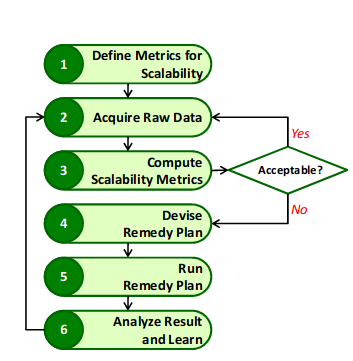
\includegraphics[width=0.7\linewidth]{figures/ServiceScalability}
	\caption{Service scalability Assuring Process from \cite{lee_software_2010}}
	\label{fig:servicescalability}
\end{figure}

\end{enumerate}

Similarly In MANO's context, the metrics defined in section \ref{Metrics} could be the basis for deciding the scalability strategy. GSM and RSM can be developed as part of the MANO's ecosystem. The scalability strategy can be a hybrid of the approaches discussed in this chapter.
GSM can also be responsible for state management of the MANO instances, that is, when scaling down a MANO, the metadata and network services managed by this MANO instance can be transferred to the next best node with sufficient resources.  
